%!TEX root = ../lectures.tex

\topic{Implicit Differentiation}

So far we have only computed derivatives of things on the form $y = f(x)$, but not everything is this nice.

Consider for example $F(x, y) = x^2 + y^2 - 1 = 0$, the equation of the unit circle.
This certainly has some kind of slope everywhere (though vertical at $(1, 0)$ and $(-1, 0)$).
How do we find these slopes?

In this particular case we can of course solve for $y$, getting $y = \pm\sqrt{1 - x^2}$, depending on which half plane we are in, and this we can differentiate using the chain rule:
\[
	y' = \pm \frac{1}{2} (1 - x^2)^{-1/2} \cdot -2 x = \mp \frac{x}{\sqrt{1 - x^2}}.
\]
We say that there are \keyword{implicit functions}\index{function!implicit}\footnote{This is actually a remarkably important idea, leading up to the Implicit function theorem in Multivariable calculus, but you'll learn more about this in a future course.} of $x$, in the sense that we can somehow extract functions in one variable $x$ describing the relation in two variables $x$ and $y$.
We can't always find these explicitly as above, however!
But we can still differentiate, as it turns out.

\begin{example}
	Differentiate implicitly $x^2 + y^2 - 1 = 0$.

	The idea is to differentiate both sides of the equation with respect to our variable $x$, meanwhile treating $y = y(x)$ as a function of $x$.
	This means that whenever we run into a $y$, we must use the chain rule:
	\begin{align*}
		\frac{d}{d x} (x^2 + y^2 - 1) = \frac{d}{d x} (0) \qquad        & \Longleftrightarrow \qquad \frac{d}{d x} (x^2) + \frac{d}{d x} (y^2) - \frac{d}{d x} (1) = 0 \\
		\Longleftrightarrow \qquad 2 x + 2 y \frac{d y}{d x} = 0 \qquad & \Longleftrightarrow \qquad \frac{d y}{d x} = - \frac{2 x}{2 y} = - \frac{x}{y},
	\end{align*}
	which if we substitute $\pm \sqrt{1 - x^2}$ for $y$ becomes
	\[
		\frac{d y}{d x} = - \frac{x}{\pm \sqrt{1 - x^2}} = \mp \frac{x}{\sqrt{1 - x^2}},
	\]
	just as above.
\end{example}

\topic{Derivatives of Inverse Functions}

Recall from previous experience that a bijective (i.e. injective (one-to-one) and surjective (onto)) function $f \colon X \to Y$ has an \keyword{inverse function}\index{function!inverse} $f^{-1} \colon Y \to X$ such that
\[
	y = f(x) \qquad \Longleftrightarrow \qquad x = f^{-1}(y)
\]
and
\[
	f(f^{-1}(y)) = y, \qquad \text{and} \qquad f^{-1}(f(x)) = x.
\]

\noindent
Using one of these so-called cancellation identities together with implicit differentiation we can find a general formula for the derivative of inverse functions:
\[
	\frac{d}{d x} \big ( f(f^{-1}(x)) \big ) = \frac{d}{d x} (x) \qquad \Longleftrightarrow \qquad f'(f^{-1}(x)) \cdot \frac{d}{d x} (f^{-1}(x)) = 1
\]
which if we solve for $\frac{d}{d x} (f^{-1}(x))$ becomes
\[
	\frac{d}{d x} (f^{-1}(x)) = \frac{1}{f'(f^{-1}(x))}.
\]

\noindent
To see why this is useful, let us attempt to differentiate (some of) the inverse trigonometric functions.

\begin{figure}[t!]
	\centering
	\begin{subfigure}{0.3\textwidth}
		\centering
		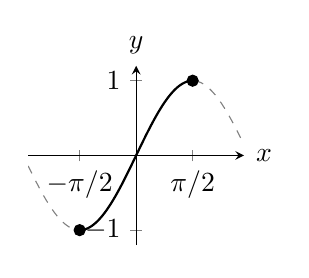
\begin{tikzpicture}
			\begin{axis}[
				scale = 0.4,
				axis x line = middle,
				axis y line = middle,
				xmin = -3,
				xmax = 3,
				ymin = -1.2,
				ymax = 1.2,
				xlabel = $x$,
				ylabel = $y$,
				xtick = {-1.571, 1.571},
				xticklabels = {$-\pi/2$, $\pi/2$},
				ytick = {-1, 1},
				yticklabels = {$-1$, $1$},
				every axis x label/.style = {
					at = {(ticklabel* cs:1.01)},
					anchor = west,
				},
				every axis y label/.style = {
					at = {(ticklabel* cs:1.01)},
					anchor = south,
				},
				]
				\addplot[
				gray,
				dashed,
				samples = 100,
				domain = -3:3,
				]{sin((x)r)};
				\addplot[
				black,
				thick,
				samples = 100,
				domain = -1.571:1.671,
				]{sin((x)r)};
				\addplot[mark=*] coordinates {(-1.571, -1)};
				\addplot[mark=*] coordinates {(1.571, 1)};
			\end{axis}
		\end{tikzpicture}
		\caption{Sine}
	\end{subfigure}
	\quad
	\begin{subfigure}{0.3\textwidth}
		\centering
		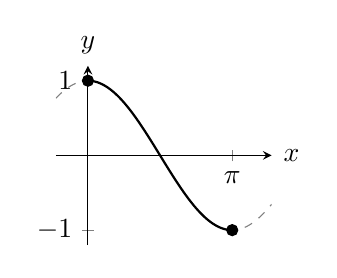
\begin{tikzpicture}
			\begin{axis}[
				scale = 0.4,
				axis x line = middle,
				axis y line = middle,
				xmin = -0.7,
				xmax = 4,
				ymin = -1.2,
				ymax = 1.2,
				xlabel = $x$,
				ylabel = $y$,
				xtick = {3.142},
				xticklabels = {$\pi$},
				ytick = {-1, 1},
				yticklabels = {$-1$, $1$},
				every axis x label/.style = {
					at = {(ticklabel* cs:1.01)},
					anchor = west,
				},
				every axis y label/.style = {
					at = {(ticklabel* cs:1.01)},
					anchor = south,
				},
				]
				\addplot[
				gray,
				dashed,
				samples = 100,
				domain = -0.7:4,
				]{cos((x)r)};
				\addplot[
				black,
				thick,
				samples = 100,
				domain = 0:3.142,
				]{cos((x)r)};
				\addplot[mark=*] coordinates {(0, 1)};
				\addplot[mark=*] coordinates {(3.142, -1)};
			\end{axis}
		\end{tikzpicture}
		\caption{Cosine}
	\end{subfigure}
	\quad
	\begin{subfigure}{0.3\textwidth}
		\centering
		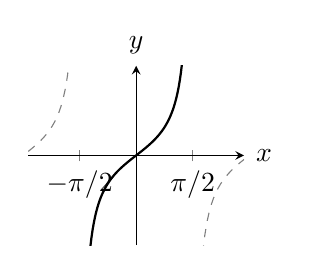
\begin{tikzpicture}
			\begin{axis}[
				scale = 0.4,
				axis x line = middle,
				axis y line = middle,
				xmin = -3,
				xmax = 3,
				ymin = -3.2,
				ymax = 3.2,
				xlabel = $x$,
				ylabel = $y$,
				xtick = {-1.571, 1.571},
				xticklabels = {$-\pi/2$, $\pi/2$},
				ytick = \empty,
				every axis x label/.style = {
					at = {(ticklabel* cs:1.01)},
					anchor = west,
				},
				every axis y label/.style = {
					at = {(ticklabel* cs:1.01)},
					anchor = south,
				},
				restrict y to domain = -4:4
				]
				\addplot[
				gray,
				dashed,
				samples = 100,
				domain = -3:3,
				]{tan((x)r)};
				\addplot[
				black,
				thick,
				samples = 100,
				domain = -1.571:1.671,
				]{tan((x)r)};
			\end{axis}
		\end{tikzpicture}
		\caption{Tangent}
	\end{subfigure}
	\caption{Restricted domains of trigonometric functions.}
	\label{lec6:inversetrig}
\end{figure}

Of course trigonometric functions are periodic and therefore not one-to-one, so in order to invert them we restrict their domains, as demonastrated in Figure \ref{lec6:inversetrig}. We therefore have
\begin{align*}
	\arcsin(\sin(x)) & = x, \qquad -\frac{\pi}{2} \leq x \leq \frac{\pi}{2}; \\
	\sin(\arcsin(x)) & = x, \qquad -1 \leq x \leq 1;                         \\
	\arccos(\cos(x)) & = x, \qquad 0 \leq x \leq \pi;                        \\
	\cos(\arccos(x)) & = x, \qquad -1 \leq x \leq 1;                         \\
	\arctan(\tan(x)) & = x, \qquad -\frac{\pi}{2} < x < \frac{\pi}{2};       \\
	\tan(\arctan(x)) & = x, \qquad -\infty < x < \infty.
\end{align*}

\noindent
We can now find the derivatives of the inverse functions, since if $y = \arcsin(x)$, we have $x = \sin(y)$, whence
\[
	\frac{d}{d x} (x) = \frac{d}{d x} \sin(y) \quad \Longleftrightarrow 1 = \cos(y) \, \frac{d y}{d x}.
\]
Since $-\pi / 2 \leq y \leq \pi / 2$, we have $\cos(y) \geq 0$, whereby the trigonometric identity $(\cos(y))^2 + (\sin(y))^2 = 1$ is equivalent with
\[
	\cos(y) = \sqrt{1 - (\sin(y))^2} = \sqrt{1 - x^2},
\]
whence
\[
	\frac{d y}{d x} = \frac{1}{\cos(y)} = \frac{1}{\sqrt{1 - x^2}}.
\]
Note that $\arcsin$ isn't differentiable at the endpoints $x = -1$ and $x = 1$ since we get division by $0$ there, and the slope approaches infinity.

Similarly for $\arccos$ we get
\[
	\frac{d}{d x} \arccos(x) = - \frac{1}{\sqrt{1 - x^2}}
\]
and for $\arctan$ we get
\[
	\frac{d}{d x} \arctan(x) = \frac{1}{1 + x^2}.
\]

\begin{exercise}
	Prove the above two claims about $\arccos$ and $\arctan$.
	Note that for the $\arctan$ function we will require the derivative of $\tan(x)$, which is quite useful and turns out to be $(\sec(x))^2 = 1 + (\tan(x))^2$.
\end{exercise}


\topic{The Natural Logarithm}

We will now \emph{define} a function $\ln(x)$, called the \keyword{natural logarithm}\index{natural logarithm} of $x$.
This definition might look quite strange, but we will show that it has the properties we expect of logarithms.

\begin{definition}[Natural logarithm]
	Take $x > 0$ and let $A(x)$ be defined as the area of the plane bounded by the curve $y = 1/t$, the $t$ axis, and the vertical lines $t = 1$ and $t = x$ (see Figure \ref{lec6:lndef}).

	The function $\ln$ is defined as
	\[
		\ln(x) = \begin{cases}
		A(x), & \text{if}~ x \geq 1 \\
		- A(x), & \text{if}~ 0 < x < 1.
		\end{cases}
	\]
\end{definition}

\begin{figure}
	\centering
	\begin{tikzpicture}
		\begin{axis}[
			scale = 1,
			axis x line = left,
			axis y line = left,
			xmin = 0,
			xmax = 4,
			ymin = 0,
			ymax = 4,
			xlabel = $t$,
			ylabel = $y$,
			xtick = {0.3, 1, 3},
			xticklabels = {$x_1$, $1$, $x_0$},
			ytick = \empty,
			every axis x label/.style = {
				at = {(ticklabel* cs:1.01)},
				anchor = west,
			},
			every axis y label/.style = {
				at = {(ticklabel* cs:1.01)},
				anchor = south,
			},
			restrict y to domain = 0:10
			]
			\addplot[
			black,
			pattern color = gray!60,
			pattern = north east lines,
			domain = 0.3:3
			]{1/x} \closedcycle;
			\addplot[
			black,
			pattern color = gray!60,
			pattern = north west lines,
			domain = 1:3
			]{1/x} \closedcycle;
			\addplot[
			black,
			samples = 100,
			domain = 0.01:4
			]{1/x};
			\addplot[mark=none] coordinates {(0.65, 0.6)} node{$\!A(x_1)\!$};
			\addplot[mark=none] coordinates {(1.5, 0.3)} node{$\!A(x_0)\!$};
		\end{axis}
	\end{tikzpicture}
	\caption{The area under $y = 1/t$.}
	\label{lec6:lndef}
\end{figure}

\noindent
From the definition it follows that $\ln(1) = 0$, $\ln(x) > 0$ if $x > 1$, and $\ln(x) < 0$ if $0 < x < 1$.
Finally since the area must increase as we move $x_0$ rightward on the figure, the function is increasing, and so injective (one-to-one).

This function has a plethora interesting properties, maybe chief amongst which is

\begin{theorem}
	If $x > 0$, then
	\[
		\frac{d}{d x} \ln(x) = \frac{1}{x}.
	\]
\end{theorem}

\begin{proof}
	If $x > 0$ and $h > 0$, then $\ln(x + h) - \ln(x)$ is the area bounded by $y = 1/t$, $y = 0$, $t = x$, and $t = x + h$, as illustrated in Figure \ref{lec6:lnareasdiff}.

	\begin{figure}[b]
		\centering
		\begin{subfigure}{0.45\textwidth}
			\centering
			\begin{tikzpicture}
				\begin{axis}[
					scale = 0.45,
					axis x line = left,
					axis y line = left,
					xmin = 0,
					xmax = 10,
					ymin = 0,
					ymax = 4,
					xlabel = $t$,
					ylabel = $y$,
					xtick = {1, 4, 7},
					xticklabels = {$1$, $x$, $x + h$},
					ytick = \empty,
					every axis x label/.style = {
						at = {(ticklabel* cs:1.01)},
						anchor = west,
					},
					every axis y label/.style = {
						at = {(ticklabel* cs:1.01)},
						anchor = south,
					},
					restrict y to domain = 0:10
					]
					\addplot[
					black,
					pattern color = gray!60,
					pattern = north east lines,
					domain = 1:7
					]{1/x} \closedcycle;
					\addplot[
					black,
					pattern color = gray!60,
					pattern = north west lines,
					domain = 1:4
					]{1/x} \closedcycle;
					\addplot[
					black,
					samples = 100,
					domain = 0.01:10
					]{1/x};
					\addplot[mark=none] coordinates {(5.5, 0.2)} node[pin=88:{$\ln(x+h) - \ln(x)$}]{};
				\end{axis}
			\end{tikzpicture}
			\caption{The area $\ln(x + h) - \ln(x)$.}
			\label{lec6:lnareasdiff}
		\end{subfigure}
		\quad
		\begin{subfigure}{0.45\textwidth}
			\centering
			\begin{tikzpicture}
				\begin{axis}[
					scale = 0.45,
					axis x line = left,
					axis y line = left,
					xmin = 0,
					xmax = 3,
					ymin = 0,
					ymax = 8,
					xlabel = $t$,
					ylabel = $y$,
					xtick = {0.2, 1.5},
					xticklabels = {$x$, $x + h$},
					ytick = \empty,
					every axis x label/.style = {
						at = {(ticklabel* cs:1.01)},
						anchor = west,
					},
					every axis y label/.style = {
						at = {(ticklabel* cs:1.01)},
						anchor = south,
					},
					restrict y to domain = 0:10
					]
					\addplot[
					black,
					pattern color = gray!60,
					pattern = north east lines,
					domain = 0.2:1.5
					]{5} \closedcycle;
					\addplot[
					black,
					pattern color = gray!60,
					pattern = north west lines,
					domain = 0.2:1.5
					]{0.6667} \closedcycle;
					\addplot[
					black,
					samples = 100,
					domain = 0.01:3
					]{1/x};
					\addplot[mark=none] coordinates {(1.5, 0.6667)} node[pin=45:{$\frac{1}{x + h}$}]{};
					\addplot[mark=none] coordinates {(1.5, 5)} node[pin=45:{$\frac{1}{x}$}]{};
				\end{axis}
			\end{tikzpicture}
			\caption{The area $\ln(x + h) - \ln(x)$.}
			\label{lec6:lnareasbound}
		\end{subfigure}
		\caption{The area under $y = 1/t$.}
		\label{lec6:lnareas}
	\end{figure}

	Clearly this area is greater than $h \cdot \frac{1}{x + h}$ and smaller than $h \cdot \frac{1}{x}$, as illustrated in Figure \ref{lec6:lnareasbound}, meaning that
	\begin{equation}\label{lec6:eq:lnbound}
		\frac{h}{x + h} < \ln(x + h) - \ln(x) < \frac{h}{x}.
	\end{equation}

	\noindent
	If we divide this through by $h$ (which is positive by assumption) we get
	\[
		\frac{1}{x + h} < \frac{\ln(x + h) - \ln(x)}{h} < \frac{1}{x},
	\]
	which by the Squeeze theorem (for one-sided limits) gives
	\[
		\lim_{h \to 0^+} \frac{\ln(x + h) - \ln(x)}{h} = \frac{1}{x}
	\]
	since
	\[
		\lim_{h \to 0^+} \frac{1}{x + h} = \lim_{h \to 0^+} \frac{1}{x} = \frac{1}{x}.
	\]

	\noindent
	Taking $h < 0$ instead (and we also need to guarantee that $x + h > 0$, so take $h$ such that $0 < x + h < x$) we get the following from Equation \eqref{lec6:eq:lnbound}:
	\[
		\frac{1}{x} < \frac{\ln(x + h) - \ln(x)}{h} < \frac{1}{x + h},
	\]
	which by the same argument yields
	\[
		\lim_{h \to 0^-} \frac{\ln(x + h) - \ln(x)}{h} = \frac{1}{x},
	\]
	so in all
	\[
		\frac{d}{d x} \ln(x) = \lim_{h \to 0} \frac{\ln(x + h) - \ln(x)}{h} = \frac{1}{x}. \qedhere
	\]
\end{proof}

\noindent
Note, by the way, that $1 / x > 0$ for all $x > 0$, which is therefore another way to see that $\ln$ is increasing.

Other interesting properties of the $\ln$ function are those we associate with logarithms:

\begin{theorem}
	If $x$ and $y$ are positive, then
	\begin{romanlist}
		\item $\ln(x y) = \ln(x) + \ln(y)$;
		\item $\ln(x / y) = \ln(x) - \ln(y)$, with the special case $\ln(1 / x) = - \ln(x)$;
		\item $\ln(x^r) = r \ln(x)$, for now assuming $r \in \Q$.\footnote{This is because we have not yet showed that arbitrary exponentials are continuous.
		If they are, we could define $\ln(x^\alpha)$ for $\alpha \in \R$ to be $\lim\limits_{r \in \Q,\, r \to \alpha} \ln(x^r)$, but we can't take the limit inside the exponential until we know it is continuous.}
	\end{romanlist}
\end{theorem}

\begin{proof}
	\fakeitem{1} Let $y > 0$ be constant.
	Then by the chain rule
	\[
		\frac{d}{d x} (\ln(x y) - \ln(x)) = \frac{y}{x y} - \frac{1}{x} = 0
	\]
	for all $x > 0$.
	Since the derivative is $0$ for all $x > 0$,
	\begin{equation}\label{lec6:eq:lnmult}
		\ln(x y) - \ln(x) = C
	\end{equation}
	must be constant by Theorem \ref{lec5:constantfunction} last lecture.
	Take $x = 1$, then $\ln(y) - 0 = C$, so $C = \ln(y)$, whence Equation \eqref{lec6:eq:lnmult} gives
	\[
		\ln(x y) = \ln(x) + \ln(y).
	\]

	\fakeitem{2} Consider
	\[
		\frac{d}{d x} \ln \Big ( \frac{1}{x} \Big ) = \frac{1}{1 / x} \cdot - \frac{1}{x^2} = - \frac{1}{x}.
	\]
	So mimicking \fakeitemref{1}, look at $\ln(1 / x) + \ln(x)$ since
	\[
		\frac{d}{d x} \Big ( \ln \big ( \frac{1}{x} \big ) + \ln(x) \Big ) = - \frac{1}{x} + \frac{1}{x} = 0,
	\]
	so $\ln(1 / x) + \ln(x) = C$ is constant, and in particular $C = 0$ (to see this, take $x = 1$).
	Therefore
	\[
		\ln \Big ( \frac{1}{x} \Big ) = - \ln(x).
	\]
	To finish the proof, take this together with \fakeitemref{1}.

	\fakeitem{3} In the same way, study
	\[
		\frac{d}{d x} \ln(x^r) = \frac{1}{x^r} \cdot r x^{r - 1} = r \cdot x^{r - 1 - r} = \frac{r}{x},
	\]
	at least for $r \in \Q$ so far, whereby
	\[
		\frac{d}{d x} \big ( \ln(x^r) - r \ln(x) \big ) = 0,
	\]
	so $\ln(x^r) - r \ln(x) = C$ for every $x$.
	Plugging in $x = 1$ gives $C = 0$, whence
	\[
		\ln(x^r) = r \ln(x). \qedhere
	\]
\end{proof}

\topic{The Exponential Function}

Since $\ln \colon \R_{> 0} \to \R$ is injective and clearly\footnote{Hopefully. Think about it!} surjective, it is bijective and therefore has an inverse function.
We call this inverse function the \keyword{exponential function}\index{exponential function}, $\exp \colon \R \to \R_{> 0}$,
\[
	y = \exp(x) \qquad \Longleftrightarrow \qquad x = \ln(y),
\]
for $y > 0$.
We already know a bit about this function.
Since $\ln(1) = 0$, we also have $\exp(0) = 1$.
Since it's an inverse, we have
\[
	\ln(\exp(x)) = x
\]
for all $x \in \R$ and
\[
	\exp(\ln(x)) = x
\]
for all $x > 0$.

Due to the last theorem we can also quickly deduce a few more properties of this function:

\begin{theorem}
	If $x$ and $y$ are any real numbers, then
	\begin{romanlist}
		\item $(\exp(x))^r = \exp(r x)$;
		\item $\exp(x + y) = \exp(x) \exp(y)$;
		\item $\exp(x - y) = \exp(x) / \exp(y)$, with the special case $\exp(-x) = 1 / \exp(x)$.
	\end{romanlist}
\end{theorem}

\begin{proof}
	We use that it is the inverse of $\ln$ alongside the previous theorem.

	\fakeitem{1} If $y = (\exp(x))^r$, then $\ln(y) = \ln(\exp(x)^r) = r \ln(\exp(x)) = rx$, whereby if we take exponents of both sides gives us $y = \exp(r x)$.

	\fakeitem{2} Take $z = \exp(x + y)$, which is equivalent with
	\[
		\ln(z) = x + y = \ln(\exp(x)) + \ln(\exp(y)) = \ln(\exp(x) \exp(y)).
	\]
	Now take exponents of both sides to get $z = \exp(x) \exp(y)$.

	\fakeitem{3} Same idea: $y = \exp(-x)$ is equivalent with
	\[
		\ln(y) = -x = - \ln(\exp(x)) = \ln \Big ( \frac{1}{\exp(x)} \Big ).
	\]
	Again the more general result follows from this together with \fakeitemref{2}.
\end{proof}
